%ju 17-Jul-22 01-Kostenrechnung.tex
$\to$ \emph{Ziel:} Kenngrößen verbessern (Produktivität,
Wirtschaftlichkeit, Umsatzrentabilität)

\textbf{Kosten- und Leistungsrechnung} (KLR) $\to$ internes
Rechnungswesen

vs.

\textbf{Buchhaltung} (FiBu) $\to$ externes Rechnungswesen

\textbf{Kosten einteilen}

\begin{enumerate}
\item
  \textbf{Vollkostenrechnung}

  \begin{itemize}
  \item
    Indirekte Kosten (Gemeinkosten, kalkulatorische Kosten)
  \item
    Direkte Kosten (Einzelkosten)
  \end{itemize}
\item
  \textbf{Kostenstellenrechnung} (Verursachergerechte Verteilung der
  Kosten: Lager, Werkstatt, Vertrieb)
\item
  \textbf{Teilkostenrechnung} (fixe Kosten, variable Kosten,
  Deckungsbeitrag)
\end{enumerate}

\section{Vollkostenrechnung}\label{vollkostenrechnung}

Vgl. Kostenrechnung, S. 79-102 (\textcite{heiser:2017:betriebsfuhrung}).

\subsection{Kosten der Werkstatt}\label{kosten-der-werkstatt}

\begin{figure}[!ht]% hier: !ht
\centering
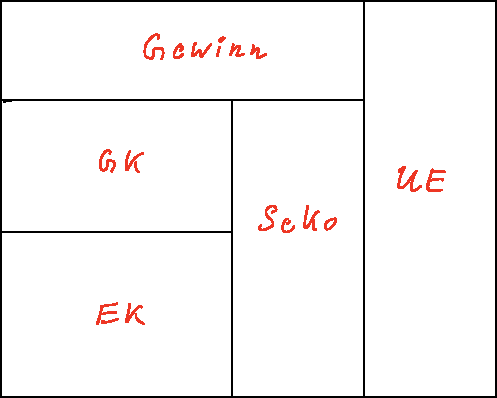
\includegraphics[width=0.4\textwidth]{images/Skizze/02_Umsatzerloese_Skizze.pdf}
\caption{Kosten und Erlöse}
%\label{fig:}%% anpassen
\end{figure}

\begin{enumerate}
\item
  \textbf{Einzelkosten} (EK), direkte Kosten (Kunden), Fertigungslöhne
  $\to$ produktiv

  \begin{itemize}
  \item
    Einzelkosten sind unmittelbar auf eine betriebliche Leistung bezogen
    und können direkt zugeordnet werden.
  \item
    $\boxed{\text{FL} = WSL \cdot Flh}$\\
  \item
    (WSL) = (StLs) Werkstattschnittlohn = Stundenlohnsatz
  \end{itemize}
\end{enumerate}

\emph{Beispiele:}

\begin{itemize}
\item
  Anschaffungskosten
\item
  Produktive Fertigungslöhne
\item
  Fertigungsmaterialien (Ersatzteile).
\end{itemize}

\begin{enumerate}
\item
  \textbf{Gemeinkosten} (GK), indirekte Kosten, Hilfslöhne (W-Aufträge)
  $\to$ unproduktiv

  \begin{itemize}
  \item
    $\boxed{\text{GK} = Seko - EK} \quad \boxed{\text{GK} = \frac{WSL \cdot GKZs}{100}}$
  \end{itemize}
\item
  \textbf{Selbstkosten} (SeKo)

  \begin{itemize}
  \item
    $\boxed{SeKo = EK + GK}$ (Einzelkosten + Gemeinkosten)
  \item
    $\boxed{SeKo = FL + GK}$ vs.~$\boxed{SeKo/h = WSL + GK/h}$
  \item
    $\boxed{SeKo_{EUR} = UE - GW} \to \boxed{SeKo_\% = 100~\% - UR_\%}$
  \end{itemize}
\item
  \textbf{Gewinn} (GW) in €

  \begin{itemize}
  \item
    $\boxed{\text{Gewinn} = UE - EK - GK} \quad \boxed{\text{Gewinn/h} = StVs - Seko/h}$
  \end{itemize}
\item
  \textbf{Umsatzerlöse} (UE in EUR), Stundenverrechnungssatz (StVs in
  EUR/h)

  \begin{itemize}
  \item
    Betrag für eine Leistung = Kostendecken + Gewinn
  \item
    $\boxed{UE = EK + GK + GW} \quad \boxed{UE = Seko + GW}$
    (Selbstkosten + Gewinn)
  \item
    $\boxed{StVs = StLs/WSL + GK + GW}$
  \end{itemize}
\end{enumerate}

\subsection{Gemeinkosten}\label{gemeinkosten}

Kosten, die einzeln nicht ermittelt werden können, da sie sich auf alle
betrieblichen Leistungen aufteilen. Sie müssen deshalb aus allen
Kostenstellen erfasst werden.

\emph{Beispiele:}

\begin{itemize}
\item
  Lohn+Gehalt (unproduktiv)
\item
  Reisekosten
\item
  Kfz (geschäftlich)
\item
  AfA
\item
  Eigenkapital (EK \% Zins)
\item
  kalkulatorische Pacht
\item
  Meisterlohn (unproduktiv)
\item
  kalkulatorische Lohn (Frau)
\item
  Vermögenswirksame Leistungen (VL)
\item
  Hilfslöhne
\item
  soziale Aufwendungen
\item
  Raumkosten
\item
  Instandhaltung
\item
  Hilfs- und Betriebsstoffe (Materialgemeinkosten)
\item
  betriebliche Steuern
\item
  Versicherungsbeiträge
\item
  Gebühren
\item
  Werbekosten
\end{itemize}

\begin{enumerate}
\item
  \textbf{Gemeinkostenzuschlagsatz} (GKZs) in \%

  \begin{itemize}
  \item
    $\boxed{\text{GKZs} = \frac{GK \cdot 100}{FL}}$
  \end{itemize}
\item
  \textbf{Kalkulatorische Kosten}

  \begin{itemize}
  \item
    aufwandsfremde Kosten
  \item
    erfassen den betriebsbedingten Aufwand
  \item
    liegen keine Rechnungen zugrunde, deshalb müssen sie kalkulatorisch
    berücksichtigt werden.
  \item
    Je nachdem, ob es sich um Kosten handelt, die in der
    Finanzbuchführung -- wenn auch in anderer Höhe -- als Aufwand
    erfasst werden oder ob es sich um Kosten handelt, die gar nicht als
    Aufwand erfasst sind (bzw. erfasst werden dürfen), spricht man auch
    von Anderskosten bzw. Zusatzkosten.
  \item
    \emph{Beispiele:}

    \begin{itemize}
    \item
      kalkulatorische Unternehmerlohn
    \item
      kalkulatorische Abschreibungen
    \item
      kalkulatorische Miete
    \item
      kalkulatorische Wagnisse
    \item
      kalkulatorische Zinsen
    \item
      kalkulatorischer Gewinn
    \end{itemize}
  \end{itemize}
\item
  \textbf{Hilfslöhne} entstehen bei Werkstattaufträgen (W-Aufträge)

  \begin{itemize}
  \item
    \emph{Beispiele:}

    \begin{itemize}
    \item
      Leerlauf
    \item
      Nacharbeiten
    \item
      Reparatur von Werkstattfahrzeuge
    \item
      Urlaub
    \item
      Feiertage
    \item
      Wartezeiten
    \end{itemize}
  \end{itemize}
\end{enumerate}

\subsection{Gewinn}\label{gewinn}

Einkommen des Unternehmers, Wagnis, Unternehmensrisiko

\textbf{Gewinnzuschlag} (GWZs) in \%
$\boxed{\text{GWZs} = \frac{GW \cdot 100}{SeKo}}$

\newpage

\subsection{Lohnkosten}\label{lohnkosten}

\textbf{Fertigungslöhne} (FL), >>produktiv<<, EK, direkte Kosten
(Kunden) - Löhne für Kundenaufträge (K-Aufträge) - Auftrag direkt dem
Kunden in Rechnung stellen - $\boxed{\text{FL} = WSL \cdot Flh}$

\emph{Beispiele:}

\begin{enumerate}
\item
  \textbf{K-Aufträge}

  \begin{itemize}
  \item
    Kundenauftrag, externe Aufträge
  \item
    \emph{Beispiel:} Wartung, Kundendienst, Reparatur von
    Kundenfahrzeugen, produktive Anteile vom Lehrlingslohn
  \end{itemize}
\item
  \textbf{I-Aufträge}

  \begin{itemize}
  \item
    interne Aufträge, innerbetrieblich (andere Abteilung des Betriebs)
  \item
    \emph{Beispiel:} Fahrzeugaufbereitung, Gebrauchtwagenreparatur,
    Überführung, Übergabedurchsicht
  \end{itemize}
\item
  \textbf{G+K-Aufträge}

  \begin{itemize}
  \item
    Garantie- und Kulanzanträge
  \item
    für Kunden ohne Berechnung, Gründe: Kulanz, Sachmängelhaftung,
    Kundenzufriedenheit gewährleisten
  \end{itemize}
\end{enumerate}

\textbf{Hilfslöhne} (HL) >>unproduktiv<<, GK, indirekte Kosten (Kunden)
- Löhne für unproduktive Stunden, die nicht unmittelbar mit der
Fertigung bzw. Reparatur zusammenhängen und von der Werkstatt getragen
werden müssen.

\emph{Beispiele:}

\begin{itemize}
\item
  allgemeine Werkstattarbeiten
\item
  Nacharbeiten, Gewährleistungen und Kulanzarbeiten, die von der
  Werkstatt getragen werden müssen
\item
  Leerlauf- und Wartezeiten
\item
  Wartung und Reparatur von firmeneigenen Fahrzeugen
\item
  Ausbildungsvergütungen
\item
  Urlaub, Feiertage
\item
  Tarifliches Urlaubsgeld
\item
  Lohnfortzahlung im Krankheitsfall
\end{itemize}

$100~\% \text{ (Lohnkosten)} = 90~\% \text{ (produktiv)} + 10~\% \text{ (unproduktiv)}$

\newpage

\textbf{Zeitlohn vs.~Leistungslohn}

\begin{enumerate}
\item
  \textbf{Zeitlohn} Fertigungslohn, produktive Arbeitszeit, Stundenlohn,
  Tariflohn

  \begin{itemize}
  \item
    \textbf{FLh} Fertigungslohnstunden
  \item
    \textbf{WSL} Werkstattschnittlohn, quer durch die Werkstatt
    \emph{Beispiel:} Lehrling, Geselle

    \begin{itemize}
    \item
      $\boxed{\text{WSL} = \frac{FL}{Flh}}$
    \end{itemize}
  \end{itemize}
\item
  \textbf{Leistungslohn} Lohn für die erbrachte Leistung

  \begin{itemize}
  \item
    \textbf{Arbeitswerte} sind Richtzeiten, die für alle normalen
    Wartungs- und Instandhaltungsarbeiten vom Hersteller festgelegt
    werden.
  \item
    \textbf{AWLs} Arbeitswertlohnsatz
  \item
    \textbf{ZELs} Zeiteinheitslohnsatz
  \item
    \textbf{Soll-AW} Vorgabe, wie viele AW muss ich in einer Stunde
    machen?
  \item
    \textbf{Ist-AW} tatsächlich erbrachte Leistung
  \item
    \textbf{Mehr-AW} Mehrleistung in AW
    $\boxed{\text{AW} = \text{Ist-AW} - \text{Soll-AW}}$
  \item
    \textbf{Vorgabezeit} Grundlage für Leistungslohn

    \begin{itemize}
    \item
      \textbf{ZE} Zeiteinheit (in Min.)
    \item
      (StVs / 60 = €/ZE x Min. = Preis (€))
    \item
      \textbf{AW} Arbeitswert (in Min.) Richtzeiten, Vorgabezeit
    \item
      \textbf{WF} Werkstattfaktor $\to$ wie viele AW/ZE in einer
      Stunde? (Soll-Leistung, Mindestleistung) (12 AW/h =
      $\frac{60}{12}$ alle 5 Min. 1 AW)
    \item
      \textbf{Leistungsfaktor} (LF) Ist-Leistung

      \begin{itemize}
      \item
        tatsächlich erbrachte Leistung je Stunde
      \item
        Leistungsfaktor = Ist-Leistung in AW / Fertigungslohnstunden
      \item
        LF = Ist-AW / FLh
      \end{itemize}
    \item
      \textbf{Leistungsgrad} (LG)

      \begin{itemize}
      \item
        $\boxed{\text{LG} = \frac{\text{Ist-AW}}{\text{Soll-AW}}}$
      \item
        Er gibt das Verhältnis von IST-Leistung zu SOLL-Leistung an.
      \end{itemize}
    \item
      \textbf{SOLL-Leistung} ist die Mindestleistung, die ein im
      Leistungslohn arbeitender Mechaniker pro Stunde erreichen soll
      (Werkstattfaktor, Normalleistung).
    \item
      \textbf{IST-Leistung} ist die tatsächlich erbrachte Leistung.
    \item
      \textbf{Leistungslohnsatz}

      \begin{itemize}
      \item
        Leistungslohnsatz = Fertigungslohn / Fertigungslohnstunden
      \item
        LLs = FL / FLh
      \end{itemize}
    \item
      \textbf{Leistungslohn} Anzahl der erreichten Arbeitswerte
      multipliziert mit der AW-Vergütung oder aus dem garantierten
      Grundlohn plus Leistungszulage.
    \end{itemize}
  \end{itemize}
\end{enumerate}

\newpage

\subsection{Kennwerte der Werkstatt}\label{kennwerte-der-werkstatt}

\begin{enumerate}
\item
  \textbf{Soll-Umsatzerlös} (Soll-UE) deckt die Selbstkosten ab

  \begin{itemize}
  \item
    Soll-UE = Seko + GW
  \end{itemize}
\item
  \textbf{Ist-Umsatzerlös} tatsächlich erwirtschaftete Umsatz
\item
  \textbf{Lohnerlöse} sind die Summe aus den produktiven
  Fertigungslöhnen, den Gemeinkosten und dem Gewinn, innerhalb einer
  Abrechnungsperiode, ohne dass die Materialkosten berücksichtigt sind.
  Lohnerlöse sind auch Erlöse aus K-, I- und G-Aufträgen
  (Gewährleistungsaufträge) ohne Material.

  \begin{itemize}
  \item
    $\boxed{\text{Lohnerlöse} = \text{produktiven Fertigungslöhnen} + \text{Gemeinkosten} + \text{Gewinn}}$
  \end{itemize}
\item
  \textbf{Wirtschaftlichkeit} (WI) Ist die Wirtschaftlichkeit größer als
  eins, so ist ein Gewinn erzielt worden. Die zwei Stellen nach dem
  Komma geben den prozentualen Gewinn, bezogen auf die Selbstkosten, an.
  Ist dieser höher als kalkuliert, so ist mehr Gewinn erzielt worden,
  als geplant wurde.

  \begin{itemize}
  \item
    $\boxed{\text{Wirtschaftlichkeit} = \frac{\text{Umsatzerlöse}}{\text{Selbstkosten}}}$
  \item
    WI = LE / Seko; WI = UE/Seko\\
  \item
    \emph{Beispiel:}
    $\text{WI} = 2,05~\% \quad 2 > 1 \to \text{ Gewinn und } 5~\% \text{ mehr als geplant}$
  \item
    WI > 1 Gewinn
  \item
    WI \textless{} 1 Verlust
  \item
    WI = 1 Kostendeckend
  \end{itemize}
\item
  \textbf{Produktivität} (PR)

  \begin{itemize}
  \item
    Gesamte Arbeitszeit (Fertigungs- + Hilfslohnstunden)
  \item
    Produktivität = Fertigungslohnstunden x 100 / Arbeitszeit
  \item
    PR = FLh x 100 / AZ
  \end{itemize}
\item
  \textbf{Umsatzrentabilität} (UR) in \%

  \begin{itemize}
  \item
    Wie viel Prozent des Umsatzes als Gewinn anfallen
  \item
    $\boxed{\text{UR} = \frac{GW \cdot 100}{UE}} \quad \boxed{\text{UR} = \frac{GW/h \cdot 100}{StVs}}$
  \end{itemize}
\end{enumerate}

\newpage

\subsubsection{Kostenindex - Stundenverrechnungssatz - AW-Vs
(Prüfung)}\label{kostenindex-stundenverrechnungssatz-aw-vs-pruefung}

\emph{3x wichtige Formeln}

\textbf{Kostenindex, Werkstattindex, Faktor} (KI) Kennzahl für die
Vorkalkulation (Werkstattindex). Er gibt an, wie viel mal mehr der Kunde
für eine Fertigungslohnstunde zu bezahlen hat, als der Monteur in dieser
Stunde verdient. (bezieht sich auf Löhne)

Beispiel: KI = 4,02 bedeutet, das der Kunde 4x mehr Zahlen muss, als der
Monteur in der Stunde verdient.

$\boxed{\text{KI} = \frac{\text{prod. Fertigungslöhne} + \text{GK} + \text{Gewinn}}{\text{prod. Fertigungslöhne}}}$

$\boxed{\text{KI} = \frac{\text{FL} + \text{GK} + \text{GW}}{\text{FL}}} \quad$
$\boxed{\text{KI} = \frac{\text{StVs}}{\text{WSL}}} \quad \boxed{\text{KI} = \frac{\text{UE}}{\text{FL}}}$

\textbf{Stundenverrechnungssatz} Arbeitspreis, der dem Kunden für eine
Stunde berechnet wird. Reparaturstunde = Fertigungslohnstunde

$\boxed{\text{StVs} = \text{KI} \cdot \text{WSL}}$

$\boxed{\text{StVs} = WSL + GK/h + GW/h} \quad \boxed{\text{StVs} = Seko/h + GW/h} \quad \boxed{\text{StVs} = \frac{\text{UE}}{\text{FLh}}}$

$\boxed{\text{StVs}_{neu} = \frac{\text{Seko}_{neu} \cdot 100~\%}{\text{Seko}_{alt}}} \quad \boxed{\Delta \text{StVs} = \text{StVs}_{neu} - \text{StVs}_{alt}}$
Erhöhung
$\boxed{\text{StVs}_\% = \frac{\Delta \text{StVs} \cdot 100~\%}{\text{StVs}_{alt}}}$

\textbf{AW-Verrechnungssatz} (Erlös je AW) dient zur Ermittlung des
Arbeitspreises (AP) für eine Arbeitsposition (Leistungslohn)

Beispiel: AW-Vs x Anzahl der AW

$\boxed{\text{AW-Vs} = \frac{\text{StVs}}{\text{WF}}} \quad \boxed{\text{AW-Vs} = \frac{\text{WSL} \cdot \text{KI}}{\text{WF}}} \quad \boxed{\text{AW-Vs} = \frac{\text{UE}}{\text{FLh} \cdot \text{WF}}}$

\newpage

\subsection{Handelswarenkalkulation}\label{handelswarenkalkulation}

\textbf{Kalkulationsarten} Vorwärts-, Rückwärts-, Differenzkalkulation

\subsubsection{Einkaufskalkulation}\label{einkaufskalkulation}

\lstset{language=Python}% C, TeX, Bash, Python 
\begin{lstlisting}[
	%caption={}, label={code:}%% anpassen
]
  BP                                           LEP                 // 100 %
- BK                                         - Rabatt       10 %                 
= BEP                           // 98 %      = ZEP                 // 100 % 
+ Skonto    2 % (in 100)                     - Skonto        2 %
= ZEP                           // 90 %      = BEP                 
+ Rabatt   10 % (in 100)                     + BK
________________________________             ______________________         
= LEP                           EUR          = BP                  EUR 
\end{lstlisting}

\begin{enumerate}
\item
  \textbf{Listeneinkaufspreis} (LEP), Ware, Angebot,
  $\boxed{BEP + \text{Skonto} + \text{Rabatt}}$
\item
  \textbf{Lieferantenrabatt} (LRa), Preisnachlass
\item
  \textbf{Zieleinkaufspreis} (ZEP), Zahlungszeitpunkt, Kauf auf Ziel
  $\boxed{BEP + \text{Skonto}}$
\item
  \textbf{Lieferantenskonto} (LSk)
\item
  \textbf{Bareinkaufspreis} (BEP), bei sofortiger Barzahlung
\item
  \textbf{Bezugskosten} (BK), Transport: Verpackung, Fracht, Zoll,
  Rollgeld
\end{enumerate}

\subsubsection{Verkaufskalkulation,
Ersatzteilkalkulation}\label{verkaufskalkulation-ersatzteilkalkulation}

\lstset{language=Python}% C, TeX, Bash, Python 
\begin{lstlisting}[
	%caption={}, label={code:}%% anpassen
]
  BP                                           LVP                 // 100 %
+ GK       20 % (auf 100)                    - Rabatt       10 %                 
= SEKO                                       = ZVP                 // 100 %
+ Gewinn    8 % (auf 100)                    - Skonto        2 %
= BVP                           // 98 %      = BVP        
+ Skonto    2 % (in 100)                     - Gewinn
= ZVP                           // 90 %      = Seko                 
+ Rabatt   10 % (in 100)                     - GKZs
________________________________             ______________________          
= LVP                           EUR          = BP                  EUR
+ UST      19 %                                                 
________________________________                        
= Rechnungsbetrag ohne Rabatt   EUR                                 
\end{lstlisting}

\begin{enumerate}
\item
  \textbf{Bezugspreis} (BP), Anschaffungskosten, Einstandspreis
  $\boxed{BEP + BK}$
\item
  \textbf{Gemeinkosten} (GK), anteilig, nicht direkt
\item
  \textbf{Selbstkosten} (SEKO), Beschaffung, Bereitstellung,
  Weiterverarbeitung
\item
  \textbf{Gewinn} Wagnis, U-Lohn
\item
  \textbf{Verkaufssonderkosten} Garantie, Provision, Kundendienst
\item
  \textbf{Barverkaufspreis} (BVP) $\boxed{BP + GK + \text{Gewinn}}$
\item
  \textbf{Kundenskonto} (KSk)
\item
  \textbf{Zielverkaufspreis} (ZVP)
  $\boxed{BP + GK + \text{Gewinn} + \text{Skonto}}$
\item
  \textbf{Kundenrabatt} (KRa)
\item
  \textbf{Listenverkaufspreis} (LVP)
  $\boxed{BP + GK + \text{Gewinn} + \text{Skonto} + \text{Rabatt}}$
\end{enumerate}

\subsubsection{Kalkulationsfaktor}\label{kalkulationsfaktor}

Vgl. Tabellenbuch S. 61 und 69 (\textcite{bell:2021:tabellenbuchKfz}).

\begin{figure}[!ht]% hier: !ht
\centering
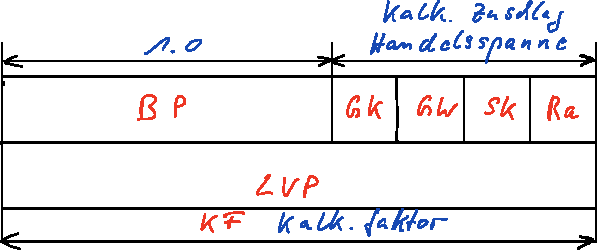
\includegraphics[width=0.6\textwidth]{images/Skizze/03_Kalkulationsfaktor_Skizze.pdf}
\caption{Kalkulationsfaktor}
%\label{fig:}%% anpassen
\end{figure}

\textbf{Kalkulationsfaktor} (KF) wie viel mal höher der (Verkaufspreis =
Listenpreis) gegenüber (Bezugspreis) bezieht sich auf das Lager,
Ersatzteil

$\boxed{KF = \frac{LVP}{BP}} \quad \to \boxed{LVP = BP \cdot KF}$

\textbf{Kalkulationszuschlag} enthält
$(GK + \text{Gewinn} + \text{Skonto} + \text{Rabatt})$ bezogen auf
(Bezugspreis)

\textbf{Handelsspanne} (HSP) unterschied zwischen (Verkaufspreis +
Bezugspreis) bezogen auf (Verkaufspreis)
$\boxed{HSP_\% = \frac{HSP \cdot 100}{LVP}}$
$\boxed{HSP_\text{EUR} = LVP - BP}$

\subsubsection{Verkauf von Tauschteilen und
Agenturwarenverkauf}\label{verkauf-von-tauschteilen-und-agenturwarenverkauf}

\textbf{Altteilesteuer} (AT-St) kauft ein Kunde ein Tauschteil und gibt
dabei sein defektes Teil (Altteil) in Zahlung, fällt Altteilesteuer an.
$\boxed{LVP \cdot 10~\% \cdot 19~\%} \quad \boxed{LVP \cdot 0,1 \cdot 0,19}$

\textbf{Agenturwaren} sind Waren, die im Auftrag und auf Rechnung einer
Fremdfirma verkauft werden (Preise inkl. Gesetzl. Ust.).

\subsubsection{Rechnungserstellung}\label{rechnungserstellung}

Kostenvoranschlag (KVA)

\textbf{Formvorschriften beachten}

\begin{itemize}
\item
  Rechnung schriftlich mit Rechnungsnummer und Leistungsdatum
\item
  Kunden- und Fahrzeugdaten wichtige aufführen
\item
  Arbeitspreis und Ersatzteilpreise detailliert aufführen
\item
  Netto-Rechnungsbetrag, Umsatzsteuer, Altteilesteuer und
  Brutto-Rechnungsbetrag einzeln aufführen.
\end{itemize}

$\text{AP} = \text{Flh} \cdot \text{StVs} \quad \text{AP} = \text{AW-Vs} \cdot \Sigma \text{AW}$

$\text{AP}_\text{Seko} = \Sigma \text{AW} \cdot \text{Seko}_{AW} \quad \text{Werkstatt AW-Preis} = \Sigma \text{AW} \cdot \text{Seko}_{AW} + \text{GW}$

\lstset{language=Python}% C, TeX, Bash, Python 
\begin{lstlisting}[
	%caption={}, label={code:}%% anpassen
]
Pos    Bezeichnung                              AW-Vs x AW           Preis
_____________________________________________________________________________
  1
  2
  3
_____________________________________________________________________________
  Summe AP                                                                EUR

                           EK                                  VP
                           80 %  20 %     100 % 24 %           124 %
                           ZEP x Rabatt = LEP + GW                      
Anzahl      Ersatzteil     (EK x 1,25)    (LEP x 1,24)       E-Preis Et-Preis
   oder
Anzahl      Ersatzteil     Rabatt (Kunden)      LVP          E-Preis Et-Preis
_____________________________________________________________________________
  1                        10 %                 (Preis x 0,9)
  1         AT-Teil
  3
_____________________________________________________________________________
  Summe ET                                                                EUR

                                                                     Preis
_____________________________________________________________________________
  AP
+ ET
+ Fremdleistung
+ Zubehör
+ Schmierstoffe
= Reparaturkosten 
+ UST                                           19 % 
+ AT-Steuer (AT-Teil x 0,1 x 0,19)
+ Agenturware (Öl)
_____________________________________________________________________________
= Rechnungsbetrag                                                         EUR
\end{lstlisting}

\newpage

\subsubsection{Lagerkosten}\label{lagerkosten}

\begin{enumerate}
\item
  Anschaffungskosten (Anfangsbestand, Warenzugang, Endbestand)

  \begin{itemize}
  \item
    $\boxed{AK = AB + WZ - EB}$
  \end{itemize}
\item
  Selbstkosten

  \begin{itemize}
  \item
    $\boxed{Seko = AK + GK}$
  \end{itemize}
\item
  Gemeinkostenzuschlagsatz

  \begin{itemize}
  \item
    $\boxed{GKZs_\% = \frac{GK \cdot 100}{AK}}$
  \end{itemize}
\item
  Gewinnzuschlagsatz (\%)

  \begin{itemize}
  \item
    $\boxed{GWZs_\% = \frac{GW \cdot 100}{Seko}}$
  \end{itemize}
\item
  Lagergewinn / Umsatzrentabilität (\% / €,Verkaufserlöse, Selbstkosten,
  Gewinn)

  \begin{itemize}
  \item
    $\boxed{GW_\% = \frac{GW \cdot 100}{VE}} \quad \boxed{GW = VE - Seko}$
  \end{itemize}
\item
  Lagerbestand

  \begin{itemize}
  \item
    $\boxed{\varnothing LB = \frac{(AB + EB)}{2}}$
  \end{itemize}
\item
  Umschlagshäufigkeit

  \begin{itemize}
  \item
    $\boxed{UH = \frac{AK}{\varnothing LB}}$
  \end{itemize}
\item
  Lagerdauer

  \begin{itemize}
  \item
    $\boxed{\varnothing LD = \frac{360~\text{Tage}}{UH}}$
  \end{itemize}
\item
  Wirtschaftlichkeit

  \begin{itemize}
  \item
    $WI = \boxed{\frac{VE}{Seko}}$
  \end{itemize}
\item
  Erlöster Kalkulationsfaktor

  \begin{itemize}
  \item
    $EKF = \boxed{\frac{VE}{AK}}$
  \end{itemize}
\end{enumerate}

\newpage

\section{Abschreibung}\label{abschreibung}

erfassen den Wertverzehr für Abnutzung und Alterung. Die AfA wird als
Aufwand gebucht, mindert Gewinn und spart Steuern.

\textbf{AfA} = Absetzung für Abnutzung

\textbf{Warum Abschreibung?}

\begin{itemize}
\item
  Verstoß gegen Bilanzwahrheit
\item
  Einkommenssteuergesetz
\end{itemize}

\textbf{Abkürzung}

\begin{itemize}
\item
  AK Anschaffungskosten
\item
  HK Herstellungskosten
\item
  ND Nutzungsdauer
\item
  RND Restnutzungsdauer
\end{itemize}

\textbf{1. lineare AfA}

\begin{itemize}
\item
  Formel: AK oder HK : Nutzungsdauer = \textbf{Abschreibung pro Jahr}
\item
  AK = AK (netto) minus Skonti, Boni und Rabatte zzgl. Transport und
  Inbetriebnahme Kosten
\item
  Nutzungsdauer = aus amtlicher AfA Tabelle
\item
  Es muss monatsgenau abgeschrieben werden
\item
  Ein Restbuchwert von 1 € muss bestehen bleiben - Bilanzklarheit
\end{itemize}

\textbf{2. degressive AfA}

\begin{itemize}
\item
  Nur wenn diese Methode bis 2010 gewählt wurde
\item
  ab 2020 wieder möglich
\item
  Formel: Restbuchwert x (lin. AfA in $\%$ x 2,5) : 100 = \textbf{AfA
  Betrag} (maximal 25 $\%$ vom Restwert!)
\end{itemize}

\textbf{3. Leistungsabschreibung}

\begin{itemize}
\item
  Möglich, wenn die Laufleistung in Stunden oder Kilometer festgehalten
  wird. Die Leistungsabschreibung kann zu einem höheren Wert als die
  lineare AfA führen.
\item
  Formel: \textbf{AfA} = (AK oder HK) : mögliche Gesamtleistung x
  tatsächliche Leistung
\end{itemize}

\textbf{4. Sonderabschreibung}

\begin{itemize}
\item
  Zerstörung oder dauerhafte Wertminderung.
\item
  Denkmalschutz Abschreibung
\item
  Abschreibung für \textbf{klein- und mittelständische Unternehmen} § 7g
  ESTG

  \begin{itemize}
  \item
    \textbf{(Gewinn \textless= € 100.000 und Betriebsvermögen \textless=
    € 235.000)} bis 40 $\%$ IAB (Investitionsabsetzbetrag)
    außerbilanziell
  \end{itemize}
\item
  Förderung Mietwohnungsbau § 7b ESTG (4 Jahre zus. 5 $\%$)
\end{itemize}

\textbf{5. geringwertige Wirtschaftsgüter GWG (netto)}

selbständig nutzbare WG (!= Drucker oder Monitore, Stuhl)

\begin{enumerate}
\item
  \textbf{Sofortaufwand}

  \begin{itemize}
  \item
    \textbf{bis \textless= € 250} sofort abzugsfähiger Aufwand
  \item
    keine Erfassung als AV - BGA (Konto Geschäftsausstattung)
  \end{itemize}
\item
  \textbf{Sofortabschreibung}

  \begin{itemize}
  \item
    \textbf{€ 250,01 bis € 800,00} - erfassen und am Jahresende voll
    abschreiben
  \end{itemize}
\item
  \textbf{Poolabschreibung}

  \begin{itemize}
  \item
    \textbf{€ 250,01 bis € 1.000,00} über 5 Jahre abschreiben.
  \end{itemize}
\item
  \textbf{Nutzungsdauer} (AfA-Tabelle)

  \begin{itemize}
  \item
    \textbf{ab € 1000,01}
  \end{itemize}
\end{enumerate}

AfA-Tabellen - Bundesfinanzministerium \footnote{\url{https://www.bundesfinanzministerium.de/Web/DE/Themen/Steuern/Steuerverwaltungu-Steuerrecht/Betriebspruefung/AfA_Tabellen/AfA_tabellen.html}}

\textbf{Berechne den Buchwert nach 6 Jahren}

\textbf{Begriffe}

\begin{itemize}
\item
  degressiv: am Anfang schnell abschreiben, Investition ankurbeln
\item
  Kombination aus linear und degressiv
\item
  Anschaffungswert
\item
  Buchwert
\item
  Nutzungsdauer
\item
  Abschreibungsbetrag
\item
  Abschreibungssatz
\end{itemize}

\lstset{language=Python}% C, TeX, Bash, Python 
\begin{lstlisting}[
	%caption={}, label={code:}%% anpassen
]
  Einkaufspreis  10.000,00
+ 5%                500,00   // Transport-, Montage und Anschlusskosten
__________________________
= AK             10.500,00   // ND: 8J

            Jahr Abschreibung Buchwert
__________________________________________           
degressiv 1J 20%     2.100,00 8.400,00 EUR
          2J 20%     1.680,00 6.720,00 EUR
          3J 20%     1.344,00 5.376,00 EUR      
          4J 20%     1.075,20 4.300,80 EUR
linear    5J         1.075,20 3.225,60 EUR
          6J         1.075,20 2.150,40 EUR
\end{lstlisting}
